% !TEX root = ../00_thesis.tex


% ------------------------------------------------------------------------------
% Global Positioning
We revisit the challenge addressed in the previous chapter: Providing end-to-end real-time guarantees in wireless cyber-physical systems (\CPS).
With the design of \DRP (\cref{ch:drp}), we demonstrated that, by leveraging synchronous transmissions (ST), it is possible to meet end-to-end deadlines between distributed tasks communicating through a multi-hop wireless network.
The principle of \DRP is to keep the tasks as independent as possible; \ie constraining their schedule as little as necessary to provide end-to-end guarantees.
% ------------------------------------------------------------------------------
% What is the problem?
Because of that maximal-flexibility principle, the guarantees that can be provided by \DRP are rather ``slow'': the minimal end-to-end deadline supported by the protocol is more than two times as large as a communication round~(\cref{sec:drp_evaluation}).
Furthermore, there is large jitter between successive task executions and message transmissions.
This does not comply well with the requirements of industrial \CPS applications, which often require short delays (the order of \ms) and benefit from negligible jitter.

\begin{figure}
  \centering
  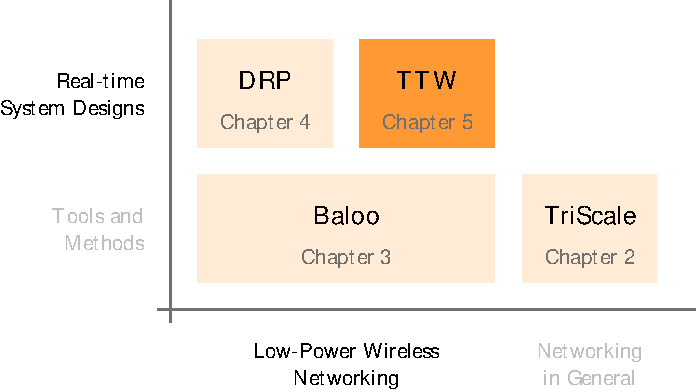
\includegraphics[scale=1]{chapter_ttw}
  \caption{This chapter presents the Time-Triggered Wireless (\TTW), a wireless \CPS design that statically co-schedules all task executions and message transfers to minimize end-to-end latency and jitter.}
  \label{fig:chapter_ttw}
\end{figure}

% ------------------------------------------------------------------------------
% Claim
Thus, in this chapter we change the design objective: Instead of focusing on flexibility, we aim for minimizing latency and jitter in the system execution.

\fakepar{Claim}
We demonstrate for that end-to-end real-time guarantees can be obtained in low-power wireless networks by leveraging the efficiency and reliability of synchronous transmissions.
In particular, this chapter presents Time-Triggered Wireless (\TTW), a design that statically co-schedules all task executions and message transfers to minimize end-to-end latency and jitter.

\pagebreak
% ------------------------------------------------------------------------------
% Corresponding reference(s)
\begin{publi}

  The material from this chapter relates to the following publication.

  \inlineRef%
  {TTW: A Time-Triggered Wireless design for CPS}%
  {Romain Jacob, Licong Zhang, Marco Zimmerling, Jan Beutel, Samarjit Chakraborty, Lothar Thiele}%
  {DATE 2018. Dresden, Germany (March 2018)}

\end{publi}
